
\chapter{Methods}

\label{Methods} 

%This chapter describes in detail the methods for whatever activities were necessary for your project – e.g., data gathering, data analysis, requirements analysis, design, implementation, testing/evaluation, etc. Your choice of methods should be discussed and justified in view of the project objectives, and with reference to the pertinent literature. Report not only what methods you applied in generic terms, but what you actually did: sufficient information about dates and details for your reader to understand how you ran your project, rather than just how one could run any similar project.  

%Report in this chapter what you did, not what you produced or found as a 
%result (which goes under Results).  
  
%Note: only use the word ‘methodology’ if you know what it means!  

%% On RELU not actually being differentiable:
%Some of the hidden units included in this list are not actually differentiable %at
%all input points. For example, the rectified linear function g (z) = max{0, z} is not
%differentiable at z = 0. This may seem like it invalidates g for use with a gradientbased
%learning algorithm. In practice, gradient descent still performs well enough
%for these models to be used for machine learning tasks. This is in part because
%neural network training algorithms do not usually arrive at a local minimum of
%the cost function, but instead merely reduce its value significantly,
%Because we do not
%expect training to actually reach a point where the gradient is 0 , it is %acceptable
%for the minima of the cost function to correspond to points with undefined gradient.
%Hidden units that are not differentiable are usually non-differentiable at only a
%small number of points.
% pg 207 Goodfellow
% This section from same book pg 475, maybe better in Context
%Another important push, still ongoing, has been towards end-to-end deep
%learning speech recognition systems that completely remove the HMM. The first
%major breakthrough in this direction came from Graves et al. (2013) who trained
%a deep LSTM RNN (see section 10.10), using MAP inference over the %frame-tophoneme
%alignment, as in LeCun et al. (1998b) and in the CTC framework (Graves
%et al., 2006; Graves, 2012).

% Batch normalization - in the context of preprocessing data for our trainng

% Feedback from Artuz Garcez relevant to Methods section
% The most important thing now is to describe clearly (with the right level of detail - not too much, not too little) the technical process (simulator, adding rain, creating the data, choice of network model and architecture/parameters)

% LC - 14 pages

%%%%%%%%%%%%%%%%%%%%%%%%%%%%%%%%%%%%%%%%%%%%%%%%%%%%%%%%%%%%%%%%%
% DATASETS
%%%%%%%%%%%%%%%%%%%%%%%%%%%%%%%%%%%%%%%%%%%%%%%%%%%%%%%%%%%%%%%%%
\section{Datasets}
Five datasets are considered Audi (\cite{geyer2020a2d2}), FordAV (\cite{agarwal2020ford}), Kitti (\cite{geiger2013vision}), Udacity (\cite{udacity2020}) and Unity, this last one being synthetic data generated specifically for this project. All provide a labelled dataset in the sense that a steering angle may be obtained for each image. In the case of Udacity simulator and Unity (SDSandbox) data, the steering angle is implicit. The remaining datasets, the steering angle may be inferred either from plain text log files, or extracted from rosbag files.

%%%%%%%%%%%%%%%%%%%%%%%%%%%%%%%%%%%%%%%%%%%%%%%%%%%%%%%%%%%%%%%%%
% Keras
%%%%%%%%%%%%%%%%%%%%%%%%%%%%%%%%%%%%%%%%%%%%%%%%%%%%%%%%%%%%%%%%%
\section{Keras}
The Keras (\cite{chollet2015keras}) deep learning API (Application Programming Interface) written in Python (\cite{van1995python}) and in this case acting as a wrapper around the machine learning library Tensorflow (\cite{abadi2016tensorflow})  was used to create, train and test models.

%%%%%%%%%%%%%%%%%%%%%%%%%%%%%%%%%%%%%%%%%%%%%%%%%%%%%%%%%%%%%%%%%
% CREATING VIDEOS
%%%%%%%%%%%%%%%%%%%%%%%%%%%%%%%%%%%%%%%%%%%%%%%%%%%%%%%%%%%%%%%%%
\section{Creating Videos}
Videos are used in this project for qualitative analysis as well as documentation. Three methods are used to create videos. The first is with the Kazam (\cite{Kazam2020}) desktop screen capture utility, which records the contents of a given display monitor. This generates video captures such as shown in Figure \ref{fig:SimTCPPred}, noting the video contains only one frame, and the three images shown in the figure represent different parts of the video. The second method was developed for this project (MakeVideo.py) and consists of parsing tcpflow logs, extracting images and predicted steering angles and creating a "side-by-side" video of the simulator being driven by the prediction engine, next to the re-created processed image presented to the network, generating video captures such as shown in Figure  \ref{fig:20201120171015_sanity_sim_network}. Examples of running the script to generate videos can be seen in a number of documented "runs", for instance \ref{app_res:36} and \ref{app_res:36}. The third method was also developed for this project (RecordVideo.py). It creates a recording at inference time with up to 3 (in case of added rain) side-by-side images in a single video. An example is shown in Figure \ref{fig:youtube20201207091932nvidia1lightrainmult_4_h5}, where most parameters (network name, rain type, predicted steering angle) are generated dynamically, and the "Intensity Multiplie" (sic) value is set in SDSandbox, hardcoded in predict\_ client.py, this python script then committed to git repository and a record of commit hash, tracking the code state at the moment recording was made, is kept in appendix \ref{res:training_and_testing_log} to make results repeatable. The concept of altering intensity multipliers to simulate glare on wet roads is in response to a suggestion by this project's supervisor (see correspondence with supervisor \ref{met:corr_arthur_2}). Examples of running the prediction engine to record can be seen in various runs, including \ref{app_res:51} and \ref{app_res:52}.

%%%%%%%%%%%%%%%%%%%%%%%%%%%%%%%%%%%%%%%%%%%%%%%%%%%%%%%%%%%%%%%%%
% tcpflow
%%%%%%%%%%%%%%%%%%%%%%%%%%%%%%%%%%%%%%%%%%%%%%%%%%%%%%%%%%%%%%%%%
\section{tcpflow}
tcpflow (\cite{tcpflowElson2013}, \cite{garfinkel2013passive}) is able to capture data packets, transmitted using the TCP (\cite{rfc793}) host-to-host protocol (which provides a process-to-process communication service) and store the data in a human readable format, such that it may be analysed and debugged. For this study, it is used to reconstruct and record data transmissions between SDSandbox and the prediction engine. A practical example is given in \ref{NetMonDebug}.

Figure \ref{fig:PredSteeringAnglestcpflowNvidia1} shows a plot of predicted and simulator steering angles. The prediction is for a single image frame sent over the network. As the simulation begins, frames are sent over the network and in this case, captured with tcpflow.

%%%%%%%%%%%%%%%%%%%%%%%%%%%%%%%%%%%%%%%%%%%%%%%%%%%%%%%%%%%%%%%%%
% git version control
%%%%%%%%%%%%%%%%%%%%%%%%%%%%%%%%%%%%%%%%%%%%%%%%%%%%%%%%%%%%%%%%%
\section{Git}
Git (\cite{chacon2014pro}) is a distributed software version control tool, also known as SCM (Source Code Management). It is used in this project to keep track of changes made to software code. A change is recorded through a \textit{commit}, which generates a unique commit hash. By comparing commits it is possible to determine how code was modified between commits. The ability to track such changes is useful to determine which parameters changed over the course of time. An example of the forensic use of Git can be seen in \ref{app_res:36}, to narrow down what code generated a well performing model.

%%%%%%%%%%%%%%%%%%%%%%%%%%%%%%%%%%%%%%%%%%%%%%%%%%%%%%%%%%%%%%%%%
% SDSandbox and the Unity Game Engine
%%%%%%%%%%%%%%%%%%%%%%%%%%%%%%%%%%%%%%%%%%%%%%%%%%%%%%%%%%%%%%%%%

\section{SDSandbox and the Unity Game Engine}
\label{met:sdsandboxAndUnity}
SDSandbox (Self Driving Car Sandbox - \cite{SDSandboxSim}) is a self-driving simulator that uses the Unity (\cite{haas2014history}) game engine to simulate 3d environment car physics, as well as terrain and lighting. SDSandbox adds a user interface with a number of circuits, and functionality to create labelled datasets consisting of images (.jpg files) and steering and throttle data (corresponding .json files). It also allows a model to be driven by a prediction engine. In addition to the Unity simulator (sdsim directory), SDSandbox also provides code (src directory) to train models (train.py) and run inferences (predict\_ client.py). A base model is supplied (models.py) that "uses NVidia PilotNet NN topology", with some modifications.  
  
Setting up the SDSandbox simulator and prediction engine is further detailed in Appendix \ref{RunningCarSimulatorForInference}.

%%%%%%%%%%%%%%%%%%%%%%%%%%%%%%%%%%%%%%%%%%%%%%%%%%%%%%%%%%%%%%%%%
% SD Sandbox and Udacity Driving Simulator Comparison
%%%%%%%%%%%%%%%%%%%%%%%%%%%%%%%%%%%%%%%%%%%%%%%%%%%%%%%%%%%%%%%%%

\section{SD Sandbox and Udacity Driving Simulator Comparison}

Two driving simulators were trialed, an earlier version of Udacity (\cite{UdacityCarSim}) and SDSandbox (see \ref{met:sdsandboxAndUnity}). Both use the Unity game engine. The former had a large user base on account of the accompanying MOOC (Massive Online Open Course), which has since started using the Unreal Engine (\cite{unrealengine}) based Carla (\cite{Dosovitskiy17}) sim (short for simulator). SDSandbox is actively developed for the open source Donkey Car autonomous vehicle (\cite{DonkeyCar2020} and used by the do-it-yourself model-scale autonomous-vehicle community DIY Robocars (\cite{DIYRobocars2020}). The majority of this community uses behavioral learning to train self-driving CNNs (see correspondence with SDSandbox main code maintainer in \ref{corr:ellerbach}).  
 
Both simulators (Figure \ref{fig:UdacitySdSandboxAutonomous}) are equivalent in the sense of acting as a testing environment for self-driving CNNs and also as a training data generator. The difference being SDSandbox is able to generate data using, in addition to manual steering, a self-driving PID (\cite{bennett1993development}) closed loop controller as implemented in PIDController.cs source code file. The process provides feedback to the simulated car, which adjusts itself on the track, based on known geometrical constraints. The feature (option \textit{Auto Drive w Rec}) makes generating training sets less laborious. The manual option (\textit{Joystick/Keyboard w Rec}) being, a simulated car must be manually steered around the track a number of times. The equivalent Udacity sim option being \textit{TRAINING MODE}.

For inference, Udacity and SDSandbox have equivalent modes. The options being   
\textit{AUTONOMOUS MODE} and \textit{NN Control over Network}. Output image sizes are 320x160 and 160x120 respectively. The Udacity sim outputs steering angles to a single comma separated values' (.csv) file, as opposed to multiple .json files. 

\begin{figure}[h!]
\centering
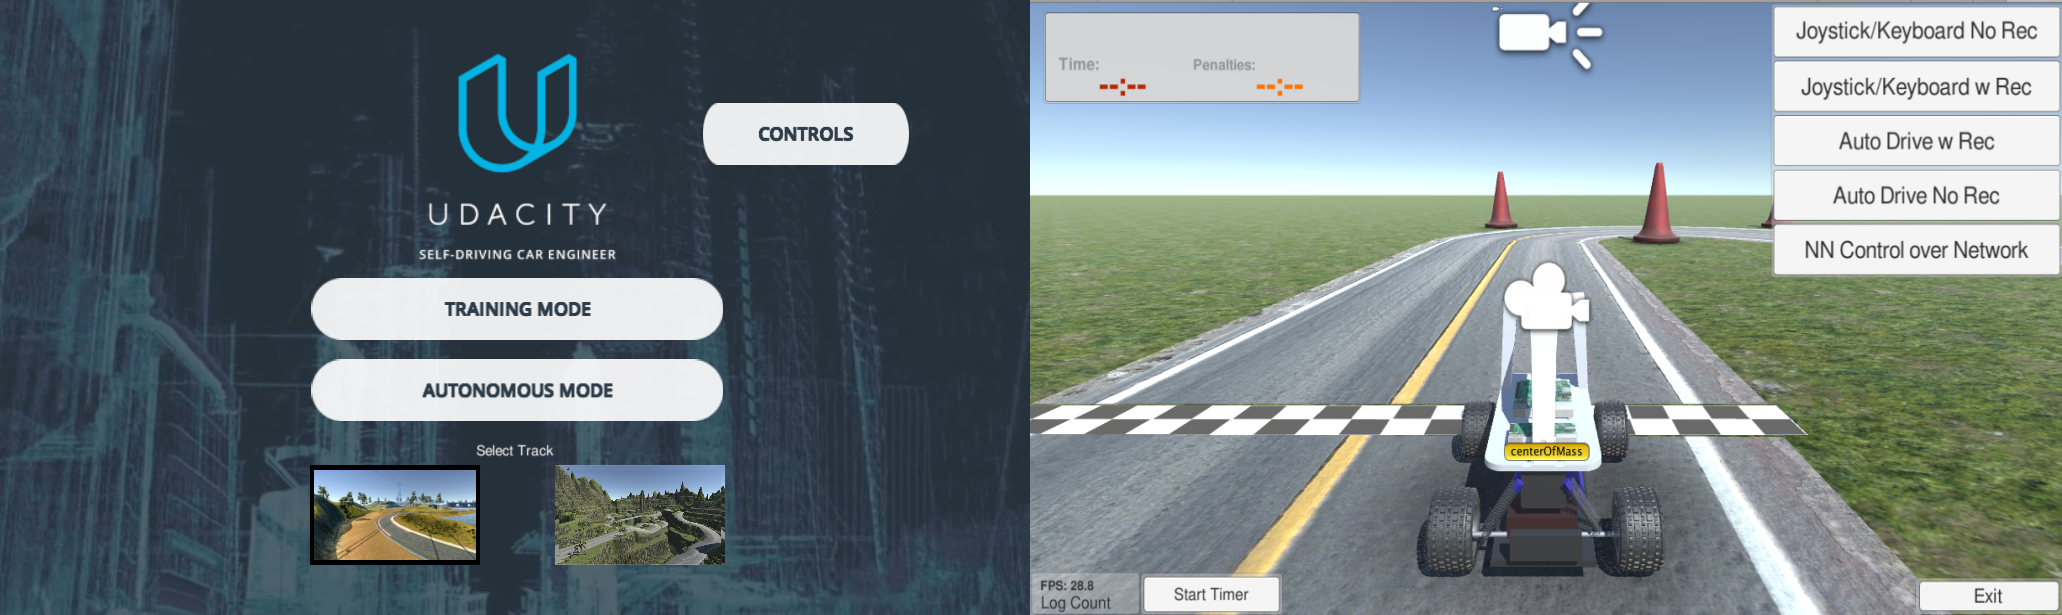
\includegraphics[width=\textwidth]{UdacitySdSandboxSim.png}
\caption{Left to right: legacy Udacity and SDSandbox Autonomous Driving Simulators}
\label{fig:UdacitySdSandboxAutonomous}
\end{figure}

Appendix \ref{AppendixA-methods} contains further notes on obtaining the source code (\ref{installing-source-code}), running the Unity Hub utility (\ref{running-unity-hub}), generating training datasets (\ref{recording-one-lap} )and running the driving simulator (
\ref{running-driving simulator})

%%%%%%%%%%%%%%%%%%%%%%%%%%%%%%%%%%%%%%%%%%%%%%%%%%%%%%%%%%%%%%%%%
% Generating Synthetic datasets - REPEATED
%%%%%%%%%%%%%%%%%%%%%%%%%%%%%%%%%%%%%%%%%%%%%%%%%%%%%%%%%%%%%%%%%

%\section{Generating Synthetic Datasets}

%\begin{itemize}
%    \item Running SDSandbox in Drive w Rec mode
%\end{itemize}

%SDSandbox has a built-in \textit{Drive w Rec} feature which enables saving of image frames generated while the simulator is running. In addition to the image, a corresponding json encoded file is also saved for every image, containing metadata which includes the reference image file name, and values for steering and throttle of simulated vehicle at the time image frame was recorded. 

%%%%%%%%%%%%%%%%%%%%%%%%%%%%%%%%%%%%%%%%%%%%%%%%%%%%%%%%%%%%%%%%%
% Adding rain to images
%%%%%%%%%%%%%%%%%%%%%%%%%%%%%%%%%%%%%%%%%%%%%%%%%%%%%%%%%%%%%%%%%

\section{Adding rain to images}
\label{methods:AddingRainToImages}
At the core of testing self-driving CNNs in the rain is the ability to add rain to images, never seen before by the network, at inference time.
Rain is added to images using the Automould (\cite{Saxena2017}) library, in turn using opencv-python, a Python port of OpenCV (\cite{mordvintsev2014opencv}), a library for Computer Vision and Machine Learning algorithms. Rain effect is created by adding lines of user defined slant, and random width. The image is then blurred by convolution with a 7x7 normalized box filter (kernel) as shown in equation \ref{eq:blurring-kernel}, taking the average of all the pixels under the kernel area and replacing the central element on the image (\cite{documentationOpenCV2020}) with the result of the convolution operation (Appendix \ref{app:rpmi}, pg 3).

\begin{equation}
\label{eq:blurring-kernel}
    K = \frac{1}{49} \begin{bmatrix} 1 & 1 & 1 & 1 & 1 & 1 & 1 \\ 
    1 & 1 & 1 & 1 & 1 & 1 & 1 \\ 
    1 & 1 & 1 & 1 & 1 & 1 & 1 \\ 
    1 & 1 & 1 & 1 & 1 & 1 & 1 \\ 
    1 & 1 & 1 & 1 & 1 & 1 & 1 \\ 
    1 & 1 & 1 & 1 & 1 & 1 & 1 \\ 
    1 & 1 & 1 & 1 & 1 & 1 & 1 \end{bmatrix}
\end{equation}
The kernel acts as a low pass filter, removing high frequency content (such as noise and edges). The image is then moved from RGB (red, green, blue) to HSL (hue, saturation, lightness) space, where the lightness values are multiplied by 0.7. This has the effect of making the image darker. The process is completed by moving the image back to RGB space. Rain types are \textit{drizzle} (a.k.a. "light", default, code checks for "heavy" and "torrential", any other non-empty string is considered drizzle/light rain), \textit{heavy}, and \textit{torrential}. Slant is defined as an angle in degrees from 0 to plus or minus 20.

% Missing an introduction discussing why this is being done
% The synthetic datasets used contain no rain. To test models with rainy images, rain must % be added. 
% To add rain to the testing images, \textit{Automold Road Augmentation Library} (\cite{Saxena2017}) is used, consisting of a Python module capable of adding rain-like effect to images. 

Figure \ref{fig:AutomoldRoadAugmentationLibrary} shows on the top row, a real-life image and on the bottom row, an image created by SDSandbox simulator. The columns from left to right have: no rain added, straight falling (0 degree slant) light, heavy with a -10 degree slant added and torrential rain with a 20 degree slant added.  
During inference (running steering predictions) the image is (in addition to same pre-processing, performed during training time) processed such that it will contain rain never seen before by the network. 
%The outcome is uncertain, given the effect of random noise on CNNs (see section TODO add section with discussion on one pixel attacks), although the flattening effect of the RGB to YUV transformation (see section TODO add section with RGB to YUV discussion) may have a desirable filtering effect.

\begin{figure}[h!]
\centering
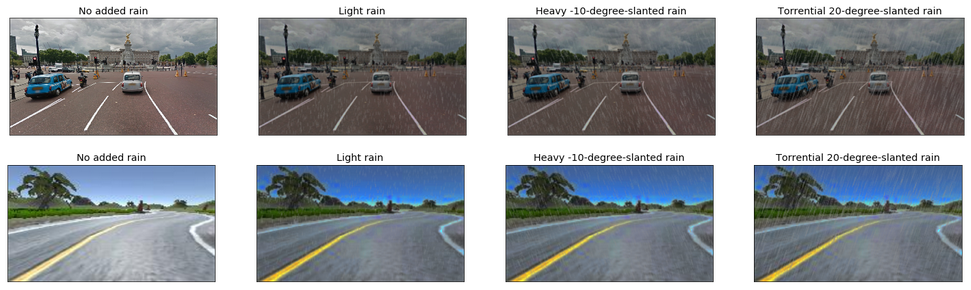
\includegraphics[width=\textwidth]{Figures/AutomoldRain.png}
\caption{Left to right: images}
\label{fig:AutomoldRoadAugmentationLibrary}
\end{figure}

%%%%%%%%%%%%%%%%%%%%%%%%%%%%%%%%%%%%%%%%%%%%%%%%%%%%%%%%%%%%%%%%%
% Data Augmentation and Pre-Processing
%%%%%%%%%%%%%%%%%%%%%%%%%%%%%%%%%%%%%%%%%%%%%%%%%%%%%%%%%%%%%%%%%

\section{Data Augmentation and Pre-Processing}

% Missing an introduction on why this is important
As discussed in \ref{Context}, data augmentation can be used to reduce overfitting, but increasing the amount of training data. The data augmentation library used in this study is adapted from \cite{Naoki2016}. Critical to the design of computer vision CNNs is the geometry of the input image. The adapted augmentation library (Augmentation.py) first resizes the image to the expected size of acquired image in the original network design. This enables code re-usability, where different networks, using different image sizes can be tested using the same code. 
Increase by a factor of 1.6 in this study.
%For the NVIDIA baseline model, assumed image capture size is 320x160 pixels, and the 200x66 pixel image presented to network is a crop containing road and excluding horizon. 
The sequence shown in figure \ref{fig:augpreproc} presents image array sizes at every step, from top left to bottom right, the image is loaded and resized (to 320 width x 160 height pixels in this case), augmented with random horizontal flip (with corresponding steering negated), random horizontal shifts (with steering adjusted by adding or subtracting 0.002 degrees per shifted pixel, random addition of shadows and random modification of brightness, concluding the augmentation part.
For the pre-processing part, the image is then cropped to remove car and horizon, resized to the dimensions determined by network design (200x66 pixels for baseline network). Crop parameters (amount of image to be removed from top and bottom sections) is network dependant and set in a configuration file (conf.py). In the example shown, 25 rows of pixels were removed from the bottom and 60 rows of pixels were removed from the top, resulting in a 320 x 75 pixel image. The image in then resized to the geometry to be presented to network, in this case 200 x 66, which is the geometry used by NaokiNet and DriveNet. Finally the image is moved from RGB to YUV space. In the RGB scheme, each pixel is represented by three channel intensities of red, green and blue. In YUV, also referred to as YCbCr (\cite{maller2020}) space, each pixel is represented by Y (luma), U (Cb - luminance value subtracted from red channel) and V (Cr - luminance value subtracted from red channel). It is a "lossy" process which degrades the data, and originally developed for colour to black and white television backward compatibility. Moving the image from RGB to YUV space has been demonstrated to give "better subjective image quality than the RGB color space", being better for computer vision "implementations than RGB due to the perceptual similarities to the human vision" (\cite{podpora2014yuv}).

\begin{figure}[ht]
 \centering 
 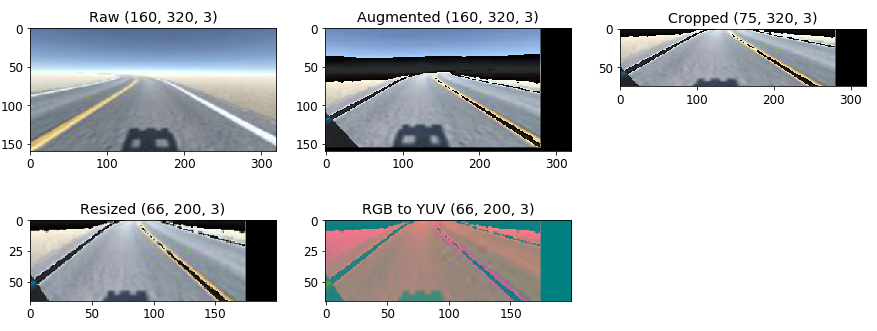
\includegraphics[width=\textwidth]{Figures/AugmentationPreProcessing.png}
 \caption{Stages of image augmentation (DriveNet and NaokiNet image geometries) and pre-processing with corresponding image array dimensions of each step}
 \label{fig:augpreproc}
\end{figure}



% Prior to presenting pixel colour channel values to the network, a number of pre-processing steps have become standard with neural network classifiers and regressors applied to computer vision.

% maybe move to appendix or results, explaining here for now

%\section{Data Augmentation}
%To avoid overfitting, the data is augmented by: cropping the %image to a height band that excluded horizon and car shadow, %resized to required model input size, converted from RGB to YUV, 
% get images from http://localhost:8890/notebooks/augument.ipynb

% \section{Training a model}

\section{Identifying rainy images with Amazon Mechanical Turk}

Amazon Mechanical Turk \cite{crowston2012amazon} is an online marketplace where jobs can be outsourced using the \textit{crowsourcing} model  (\cite{vukovic2009crowdsourcing}) which delivers a scalable workforce that may be adjusted in size as required. Mechanical Turk has been referred to as \textit{artificial artificial intelligence} (\cite{dai2011artificial}) where a task requiring human intelligence level, such as labelling an image, can be assigned to a real person, in lieu of writing  a computer algorithm capable of doing so. Mechanical Turk, launched in 2005, was instrumental in labelling the Imagenet (\cite{deng2009imagenet}) dataset which lead to advances in computer vision image recognition with a number of deep (TODO explain "deep" at some point) network architectures ( \cite{krizhevsky2012imagenet}, \cite{he2015deep}, \cite{szegedy2014going} and \cite{simonyan2015deep}). 

For this study Amazon SageMaker Ground Truth (\cite{SageMakerGroundTruthDocumentation2020}) was used. It is a wrapper for Mechanical Turk, and facilitates the process of setting up the image labelling job, especially the UI (user interface) that the labeler workforce must used.  
The aim here is to find segments of real life footage that may contain rain. The Ford AV (\cite{agarwal2020ford}) has sections labeled as "cloudy" so may contain rain. 100 images, chosen at regular intervals, the expectation being this may help narrow down the location of rainy images, if any. To test the accuracy of the service, 5 images with rain are added to the dataset. The expectation being labels for these 5 images will be "rain". 
% https://us-east-2.console.aws.amazon.com/sagemaker/groundtruth?region=us-east-2#/labeling-jobs/create
The unlabelled dataset is stored on AWS S3 (\cite{AmazonS3Documentation2020}). An "Image Classification (Single Label)" "Task type" is chosen, i.e. workers will verify if the proposed label "Rainy image" is correct. The process workflow is shown of Figure \ref{fig:amazon-ground-truth}.

\begin{figure}[ht]
 \centering 
 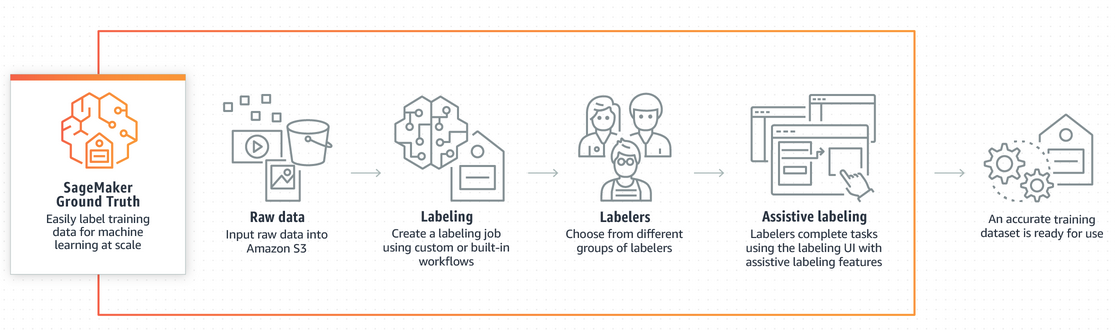
\includegraphics[width=\textwidth]{Figures/SageMakerGroundTruth.png}
 \caption{Amazon SageMaker Ground Truth workflow: a dataset is placed on Amazon S3, labeling job is created, workers label data using a labeling user interface resulting in a labeled dataset}
 \label{fig:amazon-ground-truth}
\end{figure}

\section{Training and Testing}
% TODO add the "pickle" model


\section{Deep Convolutional Neural Network Models}

In this section all network architectures used are described.

\section{NVIDIA \textit{End to End Learning for Self-Driving Cars} Network Architecture}

The NVIDIA network (\ref{NVIDIA_baseline}) is the baseline sefl-driving architecture used in this study. This comprises three (RGB channel) x 66 (height) x 200 (width) size input layer corresponding to an image presented to network. The input layer is followed by: a normalization layer generating a 3 channel 66 x 200 layer, a 24 5x5 kernel convolutional layer generating 31x98 feature maps, a 36 5x5 kernel convolutional layer generating 14x47 feature maps, a 48 5x5 kernel convolutional layer generating 5x22 size feature maps, a 64 3x3 kernel convolutional layer generating 3x20 size feature maps, a 64 3x3 kernel generating 1x18 size feature maps, a 1164 neuron flattened layer fully connected to a 100 neuron layer, fully connected to a 50 neuron layer, fully connected to a 10 neuron layer, fully connected to a one neuron output layer.  
The first 3 convolutional layers have stride equal 2 and the last 2 convolutional layers have stride equal 1. Padding is equal to zero, resulting in smaller feature maps with every convolutional layer.
The size of feature maps generated by each convolutional layer is determined with equation \ref{eq:feature_map} as described in \cite{dumoulin2018guide}:
\begin{equation}
    \label{eq:feature_map}
    n_{out}= \Big\lfloor\frac{n_{in} + 2p -k}{s} \Big\rfloor +1
\end{equation}
where $n_{out}$ is output size of convolved feature map, $n_{in}$ is input size of image or feature map, $p$, $k$ and $s$ are padding, kernel and stride size respectively.  
 
For example, to determine size of feature maps in the first convolutional layer $n_{out}=\lfloor(66+(2\times0)-5)/2\rfloor)+1=31$, $n_{out}=\lfloor(200+(2\times0)-5)/2\rfloor+1=98$. The Keras (\cite{chollet2015keras}) machine learning framework is used to build the model. The calculation for number of trainable parameters (weights) in a convolutional layer is given in equation \ref{eq:trainable_params}:
\begin{equation}
    \label{eq:trainable_params}
    n_p= m \times n \times  d \times k + d
\end{equation}
where $m$ and $n$ are the convolutional kernel dimensions, $d$ is the number of feature maps in the current layer and $k$ is the number of feature maps in the previous layer. Note $d$ is added to acccount for \textit{bias} term. For example, the number of trainable parameters for the first convolutional layer in \ref{NVIDIA_baseline} is given by $n_p = 5 \times 5 \times 24 \times 3 + 24 = 1,824$. The number of trainable parameters in a fully connected layer is given by equation \ref{eq:trainable-parmas}:
\begin{equation}
    \label{eq:trainable-parmas}
    n_p= m \times n + n
\end{equation}
where $m$ is the number of inputs in previous layer and $n$ is number of neurons in current layer. Note second term $n$ is added to account for \textit{bias} term. For example, for the first fully connected layer in \ref{NVIDIA_baseline} the number of parameters is given by $n_p = 1164 \times 100 = 1,342,092$, where the inputs are values from previous flattened layer, that is, a vectorized representation of the last convolutional layer feature maps.  
The total number of trainable parameters generated by Keras is 1,595,511. This does not agree with the total given by \cite{bojarski2016end}, who state their "network  has  about (...) 250 thousand parameters". Total memory required to store parameters assuming 32-bit float data type, is 6MB given by $1,595,511 \times 4 \div 1,024 \div 1,024$.

Since the NVIDIA model is based on work by \cite{krizhevsky2012imagenet}, "dropout" (\cite{hinton2012improving}) is assumed to have been used, with 50\% dropout probability on every layer.  
Dropout removes neurons randomly and helps prevent overfitting, where a model performs well on training data and poorly on testing data, by preventing co-adaptation, resulting in neurons that can detect useful features in the multitude of contexts it must operate, and help the network produce the correct answer.
As per correspondence with co-author(\ref{corr_with_authors} additional training hyperparameters are MSE (loss function) 
adadelta (optimizer), "learning rate: 1e-4 (but not really used in adadelta)" and 0.25 dropout.
Additional assumptions on training include: 128 example batch size, weights initialized from a zero-mean normal distribution with standard deviation 0.01 and biases mostly initialized to 1 as per \cite{krizhevsky2012imagenet}, which applied to this baseline architecture initializes all biases to 1, except in convolutional layers 1 and 5, where biases are initialized to 0. Details in source code src/models.py, nivia\_baseline function.  


% TODO need to incorporate section 5    Details of learning of Krizhesvky et al i.e.
%We trained our models using stochastic gradient descent with a batch size of 128 examples, momentum of 0.9, andw eight decay of 0.0005. ETC

% Since the weights are not initialized properly and groups of neurons end up in the same local minima, according to their (similar) initialization.
% To overcome this, you could use dropout / drop connect to break symmetry.
% https://stats.stackexchange.com/questions/181264/how-does-co-adaptation-occur-in-deep-neural-nets

% NB no reference to "Alexnet" in original or NVIDIA articles - clean up required.
%For example, in the classic Alexnet (\cite{krizhevsky2012imagenet}) architecture, with input %image size 224x224, kernel size 11, padding equal zero and stride = 4, the resulting feature %map size in the first convolutional layer is 55x55. 
%Alexnet has an input layer with dimensions 224x224x3, where 3 is the number of channels (RGB %image), the second layer has dimensions 55x55x48, the third convolutional layer has %dimensions 27x27x128 and so on. This is typical of deep network architectures, decreasing %feature map sizes with increasing number of channels as network depth increases.

\textbf{Discussion on the number of parameters required given size of dataset.}  
We also need a discussion on deep regression models as suggested by \cite{lathuilire2018comprehensive}. This is the main difference between the NVIDIA and additional models, the NVIDIA model is a regression model while the models we compare and contrast with NVIDIA are classification models built specifically for the ILSVC  competition.

\section{Training}
Discuss training, logging and training outputs, with examples of logs, history and image.


\section{Evaluation - Predicting Steering Angles}
This section discussed the evaluation benchmarks, here we discuss the evaluation environment (Unity 3D game engine) and how it was used to both generate data and evaluate the models.
We have so far a goodness of steer metric. Additionally, it would be good to have some form of noise measure, to quantify how much the image has been changed by random noise, i.e. rain.



To generated predictions \textit{on-the-fly}, the simulator is run in \textit{Auto Drive w Rec} mode. Once activated, the sends frames over the network using the OpenAI Gym (\cite{brockman2016openai} (TODO FURTHER DISCUSS PLATFORM) framework which sends packets over the network. The packets are sent from simulator using TCP (\cite{rfc793}), include packets \textbf{DESCRIBE PACKETS}.  
\textbf{DESCRIBE HANDSHAKING} \textbf{DESCRIBE TCP} 
\textbf{DESCRIBE GRAPH}
Figure \ref{fig:PredSteeringAnglestcpflowNvidia1} shows a plot of predicted and simulator steering angles. The prediction is for a single image frame sent over the network. As the simulation begins, frames are sent over the network and in this case, captured with tcpflow (\cite{garfinkel2013passive}. A log file was produced. The log file was processed (\cite{JUPYTERNOTEBOOKINAPPENDIX} and created plot. This was for one lap of the \textit{Generated Track}, similar to the track shown in Figure \ref{fig:GeneratedTrackPlusHist}. The actual processing frame rate is approximately 11fps. The y axis is flipped so the plot relates to the path taken by simulated vehicle, the first drop indicating the first right turn, the rise and sharp drop indicating the sharp right turn at the opposite end of the starting line.

\begin{figure}[ht]
 \centering 
 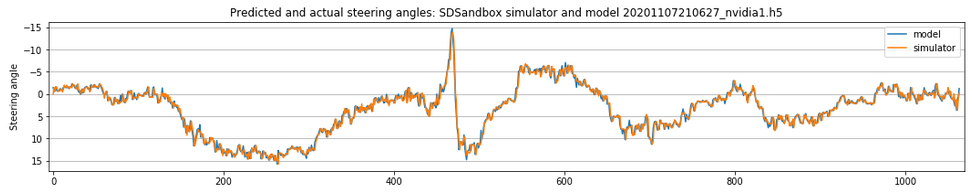
\includegraphics[width=\textwidth]{Figures/PredSteeringAnglestcpflowNvidia1.png}
 \caption{Predicted (blue) and ground-truth simulator (orange) steering angles. The simulator steering angle values in this case are obtained from data packets sent over the TCP network.}
 \label{fig:PredSteeringAnglestcpflowNvidia1}
\end{figure}

Taking this technique one step further, a video can be created using the image sent by simulator, next to the processed image presented to network. Together with the steering angle that would be used by simulator with the steering angle produced by prediction engine (predict\_client.py) which is used by the simulator.
This also can produced a metric representing \textit{goodness-of-steer}, as seen in equation     \ref{eq:goodness_of_steer}:

\begin{equation}
    \label{eq:goodness_of_steer}
    g_s(p,g) = \frac{\sum_i^N \lvert p(i)-g(i) \rvert }{N} \times n_c
\end{equation}
where $p,g$ are prediction and ground truth arrays,  $N$ is the number of predictions and $n_c$ is the normalization constant (25 in example shown, 1 for values not normalized). The sum of the absolute value of the difference between prediction and ground truth values, divided by the number of predictions multiplied by a normalization constant, is the steering error average over all predictions. This error metric is used to compare models quantitatively. For example, in Figure \ref{fig:PredSteeringAnglestcpflowNvidia1} $g_s = 0.59^{\circ}$, that is, on average the model steering is $0.59^{\circ}$ off the ground truth steering on every predicted image frame. 
%\begin{equation}
%    \label{eq:g(x,y)}
%    g(x,y) = \matchcal{H} Stopped here
%\end{equation}
TODO read up on noise models (Gonzalez)
% https://ebookcentral.proquest.com/lib/city/reader.action?docID=5573669


% From https://en.wikipedia.org/wiki/Noise_(electronics)
%In communication systems, noise is an error or undesired random disturbance of a useful information signal. The noise is a summation of unwanted or disturbing energy from natural and sometimes man-made sources. Noise is, however, typically distinguished from interference,[a] for example in the signal-to-noise ratio (SNR), signal-to-interference ratio (SIR) and signal-to-noise plus interference ratio (SNIR) measures. Noise is also typically distinguished from distortion, which is an unwanted systematic alteration of the signal waveform by the communication equipment, for example in signal-to-noise and distortion ratio (SINAD) and total harmonic distortion plus noise (THD+N) measures.

%While noise is generally unwanted, it can serve a useful purpose in some applications, such as random number generation or dither. 

%% Udacity
%% see https://arxiv.org/pdf/1912.05440.pdf
%% for discussion on using rmse as error metric - NB This relates to training a network, not the analysis of image noise.


